\documentclass[a4paper,12pt]{article}
\usepackage [left=25.4mm,top=25.4mm]{geometry}
\usepackage{amsmath}
\usepackage{amssymb}
\usepackage{graphicx}
%\usepackage{apacite}
\usepackage{url}
\usepackage{subfig}
\usepackage{csvsimple}
\usepackage{float}
\usepackage{lineno}
\usepackage[affil-it]{authblk}
\usepackage{setspace}
\usepackage{makecell} 
\usepackage{tikz}
\usepackage{csvsimple}
\usepackage{newfloat}
\usepackage{xcolor}
\usepackage{tabularx,booktabs}
\usepackage{multirow}
\usepackage{multicol}
\usepackage{array}
\usepackage{tocbasic}
\usepackage{sectsty}

\sectionfont{\fontsize{12}{15}\selectfont}
\chapterfont{\fontsize{14}{15}\selectfont}
\subsectionfont{\fontsize{10}{15}\selectfont}

\newcommand\hcancel[2][black]{\setbox0=\hbox{$#2$}%
	\rlap{\raisebox{.45\ht0}{\textcolor{#1}{\rule{\wd0}{1pt}}}}#2} 
\newcommand{\forceindent}{\leavevmode{\parindent=2em\indent}}

\DeclareFloatingEnvironment[name={Supplementary Figure},fileext=lsf,listname={List of Supplementary Figures}]{suppfigure}
\DeclareFloatingEnvironment[name={Supplementary Table},fileext=lsf,listname={List of Supplementary Tables}]{supptable}
\DeclareFloatingEnvironment[name={Supplementary Material},fileext=lsf,listname={List of Supplementary Material}]{suppmat}

\newcolumntype{P}[1]{>{\centering\arraybackslash}p{#1}}
\newcolumntype{M}[1]{>{\centering\arraybackslash}m{#1}}

\DeclareMathOperator*{\argmax}{arg\,max}
\DeclareMathOperator*{\argmin}{arg\,min}

\newcommand{\indep}{\perp \!\!\! \perp}
\renewcommand*\contentsname{TABLE OF CONTENTS}
\renewcommand{\listfigurename}{LIST OF FIGURES}
\renewcommand{\listtablename}{LIST OF TABLES}

\renewcommand{\arraystretch}{1.5}
\begin{document}
	\begin{titlepage}
		\title{HGRN Algorithm}
		\author[1]{Jarred M. Kvamme}
		\author[2]{Boyu Zhang}
		\author[1,3]{Audrey Q. Fu}
		\affil[1]{Department of Bioinformatics and Computational Biology - University of Idaho}
		\affil[2]{Department of Computer Science - University of Idaho}
		\affil[3]{Department of Mathematics and Statistical Science - University of Idaho}
		\maketitle
	\end{titlepage}
	
	
	\newpage
	\tableofcontents{}
	\addcontentsline{toc}{section}{LIST OF TABLES}
	\addcontentsline{toc}{section}{LIST OF FIGURES}
	\listoftables
	\listoffigures
	\newpage
	
	
	
	
	
	\section{Preprocessing}
	\begin{itemize}
		\item[\bf 1.1]{\textbf{Graph Initialization}: Given an attributed network $\mathcal{G}_0(E,V,X_0)$ with attribute matrix ${\bf X} =\{x_1, x_2;...;x_N\} \in \mathbb{R}^{N \times p}$ where $\bf x_i$ is the $p$-length attribute vector of node $n_i$, $E = \{ (v_i, v_j)| 1<i, j<N, i\neq j\}$ edges, and $V = \{v_i\}_{i=1}^N$ nodes/vertices, estimate an initial graph of $\bf X$ represented by the adjacency matrix ${\bf A}_0 \in \mathbb{R}^{N\times N}$ 
		\begin{itemize}
			\item[1.1.1]{\textbf{Correlations method:} Compute the correlation matrix ${\bf R}\in[0,1]^{N\times N}$ from $\bf X$. Convert the correlation matrix $\bf R$ into an adjacency matrix ${\bf A}_0$ such that 
				\[ \hat{a}_{i,j} = \begin{cases}
					1 & \text{if} \ \  r_{i,j} > \rho \\
					0 & \text{else}
				\end{cases} \] 
			where $\rho$ represents a minimum correlation threshold to consider an edge $(v_i, v_j)$ between nodes $i$ and $j$.}
			
			\item[1.1.2]{\textbf{K-neighbors method:} }
			
			\item[1.1.3]{\textbf{Precision method:}}
		\end{itemize} }
	
	\item[1.2]{\textbf{Estimate Hierarchical Structure}:} 
		
	\end{itemize}
	
	\section{Training}
	\begin{itemize}
	\item[\bf 2.1]{\textbf{Initialize HGRN Model} \\
		Input: The model takes as input the attributed graph represented by the adjacency matrix and node attribute matrix $\{{\bf A}_0, {\bf X}\}$, respectively. \\
		\\
		Parameters: \textbf{hierarchical layers} ($\ell$), \textbf{communities per layer} ($K =\{k_i\}_{i=1}^\ell$), \textbf{max training epochs} ($T$) \\
		\\
		Output: The output includes the reconstructed node attribute matrix $\hat{\bf X}$ and adjacency matrix $\hat{\bf A}$ as well as the node assignments for the \textbf{hierarchical graph} ($\mathcal{H} = \{\mathcal{G}_i\}_{i = 0}^\ell$
	}

	\item[\bf 2.2]{\textbf{For $T$ Epochs}:}
		\begin{enumerate}
			\item[2.2.1]{\textbf{Compute forward pass}: \\
			
			 \forceindent \textbf{Encoder Module}: \\
			 \forceindent \textbf{For $m$ encoder layers}: 
			\begin{enumerate}
				\item[]{\textbf{compute encoder hidden layers} \\
					We compute the first encoder layer as fully connected linear layer with activation function $\alpha_{1}$ (such as the $ReLU$, Leaky $ReLU$, Identity functions, etc). The matrix ${\bf U}_1$ represents a set of trainable weights in the linear layer. 
					\[{\bf E}_1 = \alpha_1\left({\bf X{\bf U}_1}\right)\]
					\\
					In general we compute the remaining $m-1^{th}$ hidden layers of the encoder as:
					\[{\bf E}_{m-1} = \alpha_{m-1}\left({\bf E}_{m-2}{\bf U}_{m-1}\right)\]}
				
				\item[]{\textbf{compute embedding dimension} \\
					We now compute the embedding or bottleneck dimension as a fully connected linear layer (represented by the trainable weights ${\bf U}_m$) which takes the last ($m^{th}$) hidden layer of the encoder as input. Again the function $\alpha_{m}$ represents the layer activation function.  
					\[ {\bf Z} = \alpha_{m}\left(E_{m}  {\bf U}_m\right) \]} 
			\end{enumerate}
			\forceindent \textbf{Decoder Module}: \\
			\forceindent \textbf{For $m$ decoder layers}:
			\begin{enumerate}
				\item[]{\textbf{compute decoder hidden layers.}\\
					We compute the first decoder layer as a fully connected linear layer which takes as input the embeddings $\bf Z$ and outputs the hidden decoder layer $D_1$ 
					\[ {\bf D_1} = \alpha_1({\bf ZO}_1)\]
					\\
					where $\alpha_m$ is the activation function of $m^{th}$ layer (such as the $ReLU$, Leaky $ReLU$, Identity functions, etc). $\bf Z$ is the embeddings from the bottleneck dimension and ${\bf O}_m$ is a trainable fully connected linear layer. In general, the remaining $m-1$ layers are as follows:
					
					\[{\bf D}_{m-1} = \alpha_{m-1}\left({\bf D}_{m-2}{\bf O}_{m-1}\right)\]}
				
				\item[]{\textbf{Reconstruct the input from the final decoder} layer. Here we reconstruct the input feature matrix $\hat{\bf X}$ from the final hidden layer of the decoder $D_m$. The matrix ${\bf O_m}$ represents a trainable fully connected linear layer and $\phi$ represents the output activation function. 
					\[\hat{\bf X} = \phi\left(D_m\cdot O_m\right)\]
					\\
					We also reconstruct the adjacency matrix $\hat{\bf A}$ from the embedding dimmension $\bf Z$ in the following way
					\[\hat{\bf A} = \sigma\left(Z\cdot Z^T\right) \]
					Here the function $\sigma$ denotes the sigmoid (logistic) activation function to ensure that the weights of the adjacency matrix are on the zero to one scale: $\hat{\bf A} \in [0,1]^{N\times N}$
				}
					
			\end{enumerate}
			\forceindent \textbf{Linear Classifier Layers}: \\
			\forceindent \textbf{For $\ell+1$ hierarchical layers}:
			\begin{enumerate}
				\item[]{\textbf{$\bullet$ Compute community assignment probabilities} 
					\\
					In this step we construct $\ell$ single layer linear classifiers. Each linear classifier will output the community assignments of nodes (or super-nodes) from the previous layer. The first linear classifier uses the embeddings to classify $N$ nodes to $k_1$ communities given by
					\[{\bf H}_{1} = \text{SoftMax}\left({\bf Z}{\bf W}_{1}\right) \]
					\\ 
					Where $\bf H$ is a matrix with nodes in the rows and communities in the columns. Each row of $H$ represents the probabilities for assigning a node to one of the $k_1$ communities (e.g the rows sum to 1). Here the SoftMax function is used as the layer activation function and will convert ${\bf Z}$. 
					\[{\bf H}_\ell = \begin{bmatrix}
						h_{1, 1} & \cdots & h_{1, k_\ell} \\
						\vdots  & \ddots & \vdots \\
						h_{k_{\ell - 1}, 1} & \cdots & h_{k_{\ell -1}, k_\ell} 
					\end{bmatrix}\]}
				
				\item[]{\textbf{$\bullet$ Normalize the community assignment probabilities}
					\\
					In this step the community assignment probabilities are normalized according to the method of %\cite{zhou et al} 
					\[ \hat{h}_{i,k_\ell} = \frac{\sqrt{k_{\ell-1}} \sqrt{h_{i, k_\ell}}}{\sum_i \sum_{k_\ell} \sqrt{h_{i, k_\ell}}}\]
					
					\[\hat{\bf H}_\ell = \begin{bmatrix}
						\hat{h}_{1, 1} & \cdots & \hat{h}_{1, k_\ell} \\
						\vdots  & \ddots & \vdots \\
						\hat{h}_{k_{\ell - 1}, 1} & \cdots & \hat{h}_{k_{\ell -1}, k_\ell} 
					\end{bmatrix}\]
				}
				
				
				\item[]{\textbf{$\bullet$ compute community assignment matrix} \\ 
					The community assignment matrix is a boolean matrix which represents the community assignment of a node or super node such that the value 1 at the $k_\ell^{th}$ position if a node is assigned to community $k_\ell$ and zero otherwise. This matrix can be obtained by taking the argument maximum over the rows of community assignment probabilities ${\bf H}_\ell$ for the $\ell^{th}$ hierarchical layer.  
					\[{\bf C}_{\ell} = g({\bf \hat{H}}_{\ell}) \ \text{where} \ \  g(\hat{h}_{i,k_\ell}) = 
					\begin{cases} 1 & \ \text{if} \ \ \hat{h}_{i,k_\ell} = \argmax_{k_\ell} \hat{\bf h}_i \\ %\in \mathcal{C}^{\ell}_{k_\ell} \\
						0 & \text{else} %\ v_i \not\in \mathcal{C}^{\ell}_{k_\ell}
					\end{cases}\]}
				
				\item[]{\textbf{$\bullet$ Compute community labels} \\
					For each hierarchical layer $\ell$ we may compute the community assignment labels. Consider a two-layer hierarchy, the community assignment labels $\mathbb{S}_1$ from assigning $N$ nodes in the bottom layer to $k_1 < N$ nodes in the super layer is given as 
					\[\mathbb{S}_1 = \argmax_{k_1} {\bf C}_1 \]
					
					more generally, the labels from assigning nodes in layer $\ell - 1$ to layer $\ell$ is given as:
					
					\[ \mathbb{S}_\ell = \argmax_{k_\ell} {\bf C}_{\ell}\]}
				
				\item[]{\textbf{$\bullet$ Compute input to the next classifier:}  \\
					Before we can proceed to the linear classifier corresponding to the $\ell^{th}$ hierarchical layer we need to compute its input as the centroids of the previous layer a linear. Thus the matrix ${\bf \tilde X}_\ell$ represents the centroids computed from assigning nodes in previous layer $\ell - 1$ to the communities represented by nodes in the current layer $\ell$. Thus the input of the second classifier is computed as the centroids of the first classifier defined by the linear combination of the embeddings and the community assignment matrix: 
					\[ {\bf \tilde X}_{(1)} = g_1\left({\bf Z}^T {\bf C}_{1}\right)^T\] 
					\\
					In general this can be written as: 
					\[ {\bf \tilde X}^{(\ell)} = g_\ell\left({\bf Z}_{\ell}^T {\bf C}_{\ell}\right)^T\] 
					\\
					Here the function $g$ represents the layer activation function. \\
					
					We may also compute the adjacency matrix corresponding to the sub-graph formed by assigning the $N$ original nodes to $k_1$ communities. We consider two approaches for computing ${\tilde{\bf A}^{\ell}}$. 
					\begin{itemize}
						\item[$\rightarrow$]{The first approach employs the \textbf{dot-product decoder} described by \cite{kipf2016variational,zhou2023community}. For the first linear classifier the reconstructed adjacency matrix is decoded from the embeddings:
							\[ {\bf \tilde A}^{(1)} = \sigma \left( {\bf Z}\bf{Z}^T \right) \]
						For layers $\ell > 1$ the reconstructed adjacency matrix is the dot product decoding of the centroids such that:
						\[\tilde{\bf A}^{(\ell)} = \sigma\left({\bf \tilde X}^{(\ell)}\cdot [{\bf \tilde X}^{(\ell)}]^T\right) \]
						}
						\item[]
						\item[]
						\item[$\rightarrow$]{
						For the second method first consider a two-layer hierarchical network where the first layer contains $N$ nodes $V = \{v_i\}_{i=1}^N$ and the super-layer is represented by a graph with $k_1<N$ super-nodes $\mathcal{\bf S} = \{\mathcal{S}_1, \mathcal{S}_2, \cdots \mathcal{S}_{k_1}\}$. Each super-node $\mathcal{S}_i$ is the community representation of the nodes the bottom layer such that $\mathcal{S}_i = \{v_j\}_{j=1}^{N_i}$ where $N_i$ represents the number of nodes in the $i^{th}$ community. The second approach follows from the Louvain algorithm \cite{blondel2008fast} in which an edge between two super-level nodes is represented as the sum of the edge weights for the edges connecting the nodes in community $i$ to community $j$. 
						
						\[\mathcal{E}_{ij} = (\mathcal{S}_i, \mathcal{S}_j) = \sum_{v_i \in \mathcal{S}_i, v_j \in \mathcal{S}_j}  (v_i, v_j) \]
						
						where $\mathcal{E}_{ij}$ represents the edge between super nodes $\mathcal{S}_i$ and $\mathcal{S}_j$ and the sum is over all pairs of connecting them. Given the community matrix $\bf C$ which maps the assignments of the nodes in $\bf V$ to the communities in $\mathcal{\bf S}$ the adjacency for any super level graph can be easily computed as 
						
						\[ \tilde{\bf A} = {\bf C^T}{\bf A}{\bf C} \] 
						
						Where $\bf A$ represents the bottom level graph with $N$ nodes and $\tilde{\bf A}$ represents the super-level graph with $M$ nodes.
						}
					\end{itemize}
					}
					
			\end{enumerate}
			
			
			\item[2.2.2]{\textbf{Compute Loss}: \\
				\textbf{For $L$ hierarchical layers}
			\begin{enumerate}
				\item[]{compute the loss function \\
					
					The total loss function consists of two primary components: The reconstruction loss $\mathcal{L}_R$ and the modularity $\mathcal{L}_M$
					\[\mathcal{L}_{\text{Total}} = \mathcal{L}_R - \gamma\mathcal{L}_M \]
					where $\gamma$ denotes a tuning parameter for the modularity component. The primary objective of fitting is to maximize the modularity component while minimizing the reconstruction loss. \\
					
					The reconstruction loss is composed of two reconstruction losses. The first is the binary cross entropy (BCE) loss of the input adjacency and reconstructed adjacency matrix given by: 
					\[L_{R_A} = \frac{1}{\sum_i\sum_j a_{ij}} \sum_{a_{ij}\in {\bf A}} -(a_{ij} \cdot\log(\hat{a}_{ij})+(1 - a_{ij})\cdot\log(1 - \hat{a}_{ij})) \]
					Which aims to ensure that the reconstruction loss maintains the structure of the input graph. The second is the frobenius loss for the input node attribute matrix 
					\[L_{R_X} = ||{\bf X} - \hat{\bf X}||_F = \sum_i^N \sum_j^N \left(x_{ij} - \hat{x}_{ij}\right)^2 \]
					which aims to ensure that the original node features can be recovered. 
					
					\[L_M = \sum_{i = 1}^{\ell} \mathcal{L}_i =  \sum_{i=1}^\ell \frac{1}{4\mu_\ell}Tr\left(\hat{\bf P}_\ell {\bf B_\ell} \hat{\bf P}_\ell\right)\]
					where\\
					\[{\bf B_\ell} = {\bf \tilde A}^{(\ell)}_{i,j} - \frac{d(v_i)\cdot d(v_j)}{2\mu_\ell}\]
					
					\[\mu_\ell = \frac{1}{2}\sum_i^{k_\ell} \sum_j^{k_\ell} {\bf \tilde A}^{(\ell)}_{ij}\]
					}
			\end{enumerate}
			}
			\item[2.2.3]{\textbf{Compute backward pass:}} \\
			\textbf{For ${\bf X}_0$, $\hat{\bf A}_0$ } 
			\begin{enumerate}
				\item[]{compute parameter gradients 
					\[\triangledown_\theta \mathcal{L} =  \frac{\partial\mathcal{L}}{\partial {\bf \theta}} \ \ \forall \theta \in {\bf \Theta}\]}
				
				\item[]{update all parameters $\theta \in {\bf \Theta}$}  
			\end{enumerate}
			
		}
		\end{enumerate} 
	
	\end{itemize}
	
	

\newpage
\appendix
\begin{table}[!ht]
	\centering
	\caption{Notation and explanations}
	\begin{tabular}{p{2cm}|p{3cm}|p{10cm}}
		\toprule[0.08cm]
		\bf Symbol & \centering \bf Dimension & \bf Explanation \\
		\cmidrule(lr){1-3}
		$\ell$ & & The number of super layers in the hierarchy \\
		
		$L$ & & The total number of layers in the hierarchy \\
		
		$N$ & & The number of nodes in the attributed graph \\
		
		$p$ & & The number of attributes \\
		
		$m$ & & The number of hidden encoding layers \\
		
		$d_m$ & & The column dimension of the $m^{th}$ hidden layer \\
		
		$k_\ell$ & & The number of nodes in the $\ell^{th}$ super layer \\
		
		$d(\cdot)$ & & A function which returns the degree of a node \\
		
		$\mu_\ell$ & & The number of edges in $\ell^{th}$ super layer network $\mathcal{G}_{\ell}$ \\
		
		${\bf A}_0$ & $ \in \mathbb{R}^{N \times N}$ & The input estimate of the adjacency matrix \\
		
		${\bf X}$ &$\in \mathbb{R}^{N \times p}$ & The input node-attribute matrix \\
		
		${\bf E}_{m-1}$ & $\in \mathbb{R}^{N \times d_{m-1}}$ & The ${m-1}^{th}$ hidden layer of the encoder module\\
		
		${\bf D}_{m-1}$ & $\in \mathbb{R}^{N \times d_{m-1}}$ & The ${m-1}^{th}$ hidden layer of the decoder module\\
		
		${\bf U}_{m-1}$ & $\in \mathbb{R}^{d_{m-2}\times d_{m-1}}$ & the weights corresponding to the ${m-1}^{th}$ hidden layer of the encoder module \\
		
		${\bf O}_{m-1}$ & $\in \mathbb{R}^{d_{m-2}\times d_{m-1}}$ & the weights corresponding to the ${m-1}^{th}$ hidden layer of the decoder \\
		
		${\bf Z}_{\ell}$ & $\in\mathbb{R}^{k_\ell \times d_m}$ & the embeddings belonging to the $\ell^{th}$ hierarchical layer \\
		
		${\bf W}_\ell$ & $\in\mathbb{R}^{d_m \times k_{\ell + 1}}$ & The weights corresponding to the linear classifier in the $\ell^{th}$ hierarchical layer\\
		
		${\bf H}_\ell$ & $\in\mathbb{R}^{k_{\ell-1} \times k_\ell}$ & The assignment probabilities of the $\ell^{th}$ hierarchical layer \\
		
		${\bf C}_\ell$ & $\in\mathbb{R}^{k_{\ell-1} \times k_\ell}$ & The assignment matrix of the $\ell_{th}$ hierarchical layer \\
		
		${\bf \tilde X}^{(\ell)}$ & $\in\mathbb{R}^{k_\ell \times q_m}$& The centroids of the communities in the $\ell^{th}$ hierarchical layer \\
		
		${\bf \tilde A}^{(\ell)}$ & $\in\mathbb{R}^{k_\ell \times k_\ell}$& The computed adjacency matrix corresponding to the $\ell^{th}$ hierarchical layer \\
		
		${\bf B}_\ell$ & $\in\mathbb{R}^{k_\ell \times k_\ell}$ & The modularity matrix for the $\ell^{th}$ hierarchical layer \\
		
		\bottomrule[0.08cm]
	\end{tabular}
\end{table}

\newpage

\begin{figure}
	\caption[HGRN schematic]{Proposed HRGN schematic. Example represents a model constructed for a hierarchy with $\ell = 2$ super layers.}
	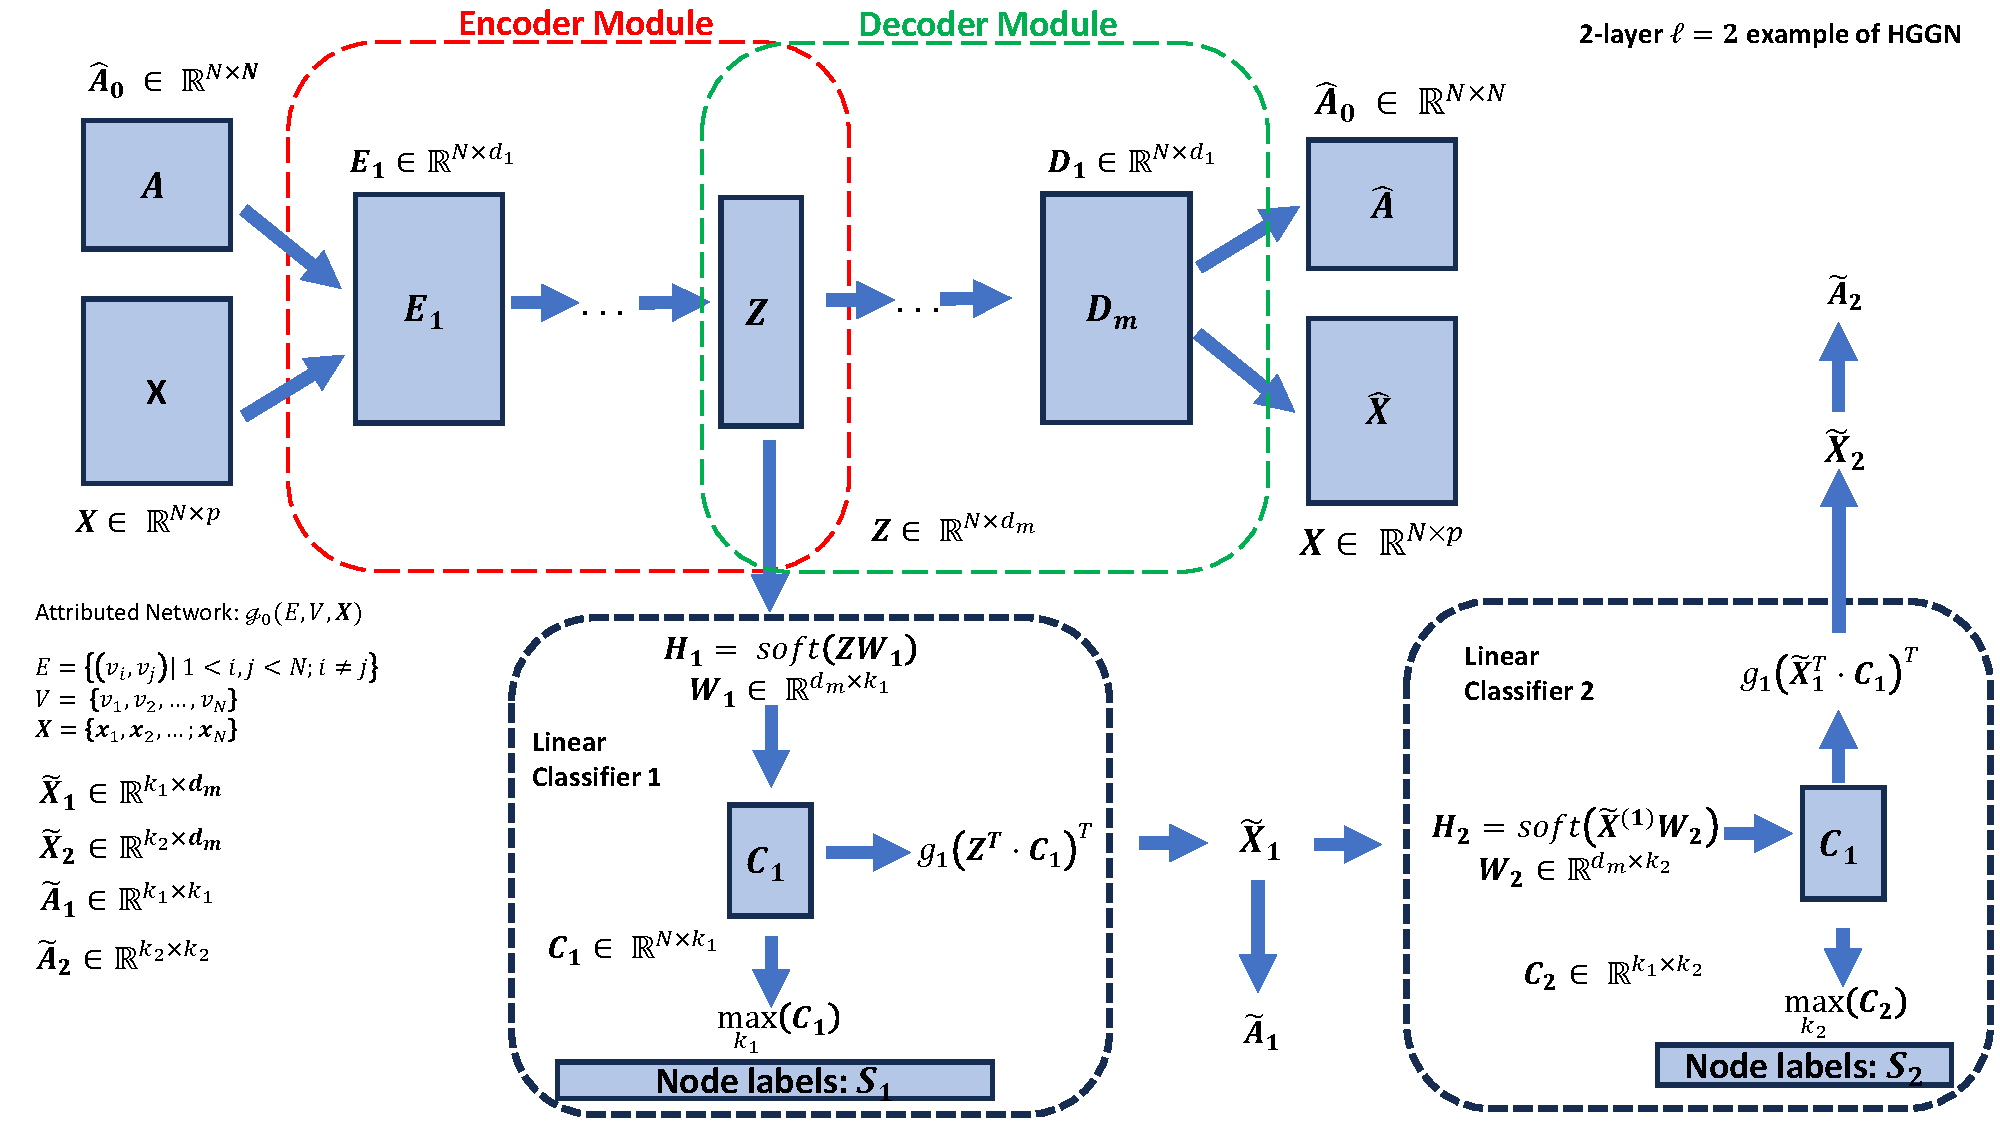
\includegraphics[scale = 0.5]{C:/Users/Bruin/Documents/GitHub/HGRN_repo/HGRN_pseudocode/HGRN_schematic.pdf}
\end{figure}
	
	
	
	
	
	
	
	
	
	
	
	
	
	
	
	
	
	
	
	
	
	
	
	
	
	
	
	
	
	
	
	
	
	
	
	\clearpage
	\newpage
	
	\bibliographystyle{unsrt}
	\bibliography{pseudocode_bibs}
	
	
	
	
	
	
\end{document}